\documentclass[a4paper,12pt]{article}
\usepackage{array}
\usepackage{listings}
\usepackage{graphicx}
\graphicspath{ {./images/} }

\setlength{\tabcolsep}{18pt}
\renewcommand{\arraystretch}{1.2}


\begin{document}
\title{Zusammenfassung Betriebssysteme}
\author{Mathis Hermann}
\date{\today}
\maketitle
Diese Zusammenfassung ist basierend auf den gegebenen Unterlagen. Alle Angaben ohne Gewähr. Weitergabe und Verbreitung erlaubt nur mit expliziter Genehmigung.

\paragraph{Inhalte des Moduls}
\begin{itemize}
\item Der grundlegende Aufbau eines Betriebssystems
\item Die Aufgaben der einzelnen Betriebssystem-Moduel und Abgrenzung voneinander sowie von darauf aufbauenden Modulen ( Applikationen, Datenbanken, Middleware-Komponenten)
\item Vor- und Nachteile bzw. Einsatzgebiete verschiedener Typen von Betriebssystemen und Zuordnung anhand gegebener Vorgaben
\item Überblick über aktuelle Forschungs- und Entwicklungsschwerpunkte im Bereich Betriebssysteme
\end{itemize}

\section{Einführung Betriebssysteme}
Ein Betriebssystem ist die Software, die die Verwendung (den Betrieb) eines Computers ermöglicht. Es verwaltet Betriebsmittel wie Speicher, Ein- und Ausgabegeräte und steuert die Ausführung von Programmen.

\paragraph{Definitionen}
\begin{itemize}
\item Kernel -- Betriebssystemkern; verwaltet Hardware des Computers
\item Grundlegende Programme -- dienen dem Start des BS und dessen Konfiguration
\end{itemize}

\subsection{Klassifizierung von Betriebssystemen}
Nach Kriterien:
\begin{itemize}
\item Nutzeranzahl:
    \begin{itemize}
    \item Single-User-BS
    \item Multi-User-BS
    \end{itemize}
\item Anzahl unabhängiger Aktivitäten:
    \begin{itemize}
    \item Single-Tasking-BS
    \item Multi-Tasking-BS
    \end{itemize}
\item Kommunikation mit der Umwelt:
    \begin{itemize}
    \item Stapelverarbeitung (Batchbetrieb)
    \item Interaktives BS
    \item BS für autonome Systeme
    \end{itemize}
\item Verteilung:
    \begin{itemize}
    \item Lokales BS
    \item Verteiltes BS
    \end{itemize}
\item Zielarchitektur / Einsatzzweck:
    \begin{itemize}
    \item Serverbetriebssystem
    \item Eingebettetes BS
    \item Echtzeitsystem | Mainframe-BS
    \item BS für Personal Computer
    \item BS für Smart Card
    \item BS für Ausbildung / Lehre
    \end{itemize}
\end{itemize}

\paragraph{Systeme in Computern}
\begin{itemize}
\item Echtzeitsysteme auf Prozessrechnern
\item Embedded-Systeme (e.g. Set-Top-Boxen, Waschmaschinen)
\item Auf normalen PCs, Tablets, Smartphones
\item Mehrprozessorsysteme auf Hosts und Grossrechnern
\end{itemize}

\subsection{Abstraktion}
\begin{itemize}
\item ungestörte Programmabarbeitung $ \rightarrow $ Prozess
\item unendlich grosser Speicher, Files $ \rightarrow $ Speicherverwaltung
\item private Maschine $ \rightarrow $ Zugriffsschutz., Datensicherheit
\end{itemize}

\paragraph{Prozess} Programm bei der Ausführung. Anforderungen an Prozessmanagement:
\begin{itemize}
\item Zeitzuteilung
\item Signalisierung von Ereignissen (e.g. I/O)
\item Vermeidung von Zugriffskonflikten -- Synchronisation
\end{itemize}


\paragraph{Speicherverwaltung}
\begin{itemize}
\item Verwendung von Speicher ohne Berücksichtigung der Grösse des physikalischen Speichers
\item Nur Teile laufender Programme werden im physikalischen Speicher gehalten
\item Der Rest befindet sich auf dem Sekundärspeicher: adressierbarer Speicher $\rightarrow$ Arbeitsspeicher
\end{itemize}

\begin{center}
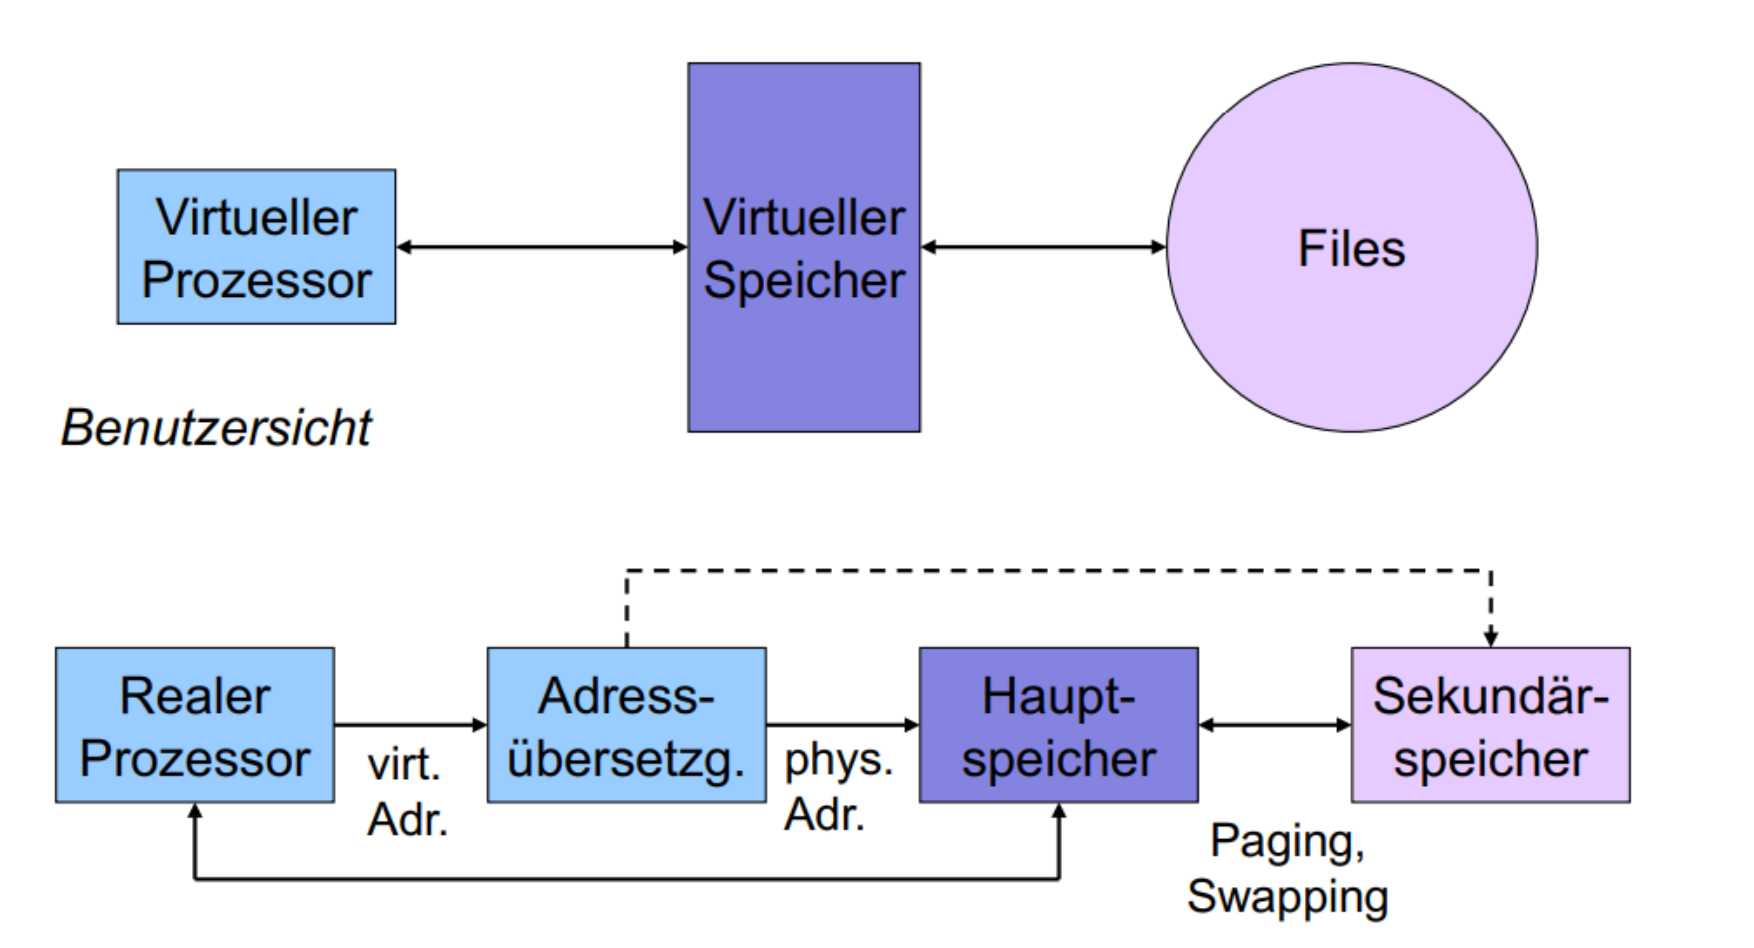
\includegraphics[width=12cm]{img/01_speicher.png}
\end{center}


\paragraph{Datenschutz und Sicherheit}
\begin{itemize}
\item Access Control
\item Information flow control
\item Authentizität -- Quelle der Information
\item Integrität -- keine Verfälschungen
\item Verfügbarkeit
\end{itemize}

\paragraph{Eigenschaften}
\begin{itemize}
\item Funktionale Eigenschaften
    \begin{itemize}
    \item Authentisierung, Verschlüsselung
    \item Informationsmanagement
    \item Kommunikationsmanagement
    \item Fahrzeug / Verkehrsmanagement
    \end{itemize}
\item Nichtfunktionale Eigenschaften
    \begin{itemize}
    \item Sicherheit
    \item Korrektheit
    \item Echtzeitfähigkeit
    \item Sparsamkeit
    \item Verfügbarkeit
    \item Skalierbarkeit
    \item Offenheit
    \item Robustheit
    \end{itemize}
\end{itemize}

\subsection{Interaktionen mit dem Betriebssystem}
Paradigmen:
\begin{itemize}
\item Vorwiegend textorientiert -- Konsole, Shell, Eingabeaufforderung
\item Grafische Oberfläche -- Windows, KDE, Windowmaker
\end{itemize}

Persönliche Vorliebe, keine Definition, was besser ist.

\subsection{Architekturen von Betriebssystem}
BS gehören zu den komplexesten Softwaresystemen. Durch Lesen des Programmcodes kaum zu verstehen. Durch Reduktion der möglichen Kommunikationsbeziehungen zwischen Komponenten Übersicht schaffen.

\paragraph{Monolith}
\begin{itemize}
\item The Big Mess
\item Jede Routine, Funktion etc. darf jede andere im System aufrufen
\item unübersehbare Vielfalt potentieller Kommunikationsbeziehungen
\item Kein \emph{Information Hiding}
\item BS = Sammlung an Funktionen
\item Typisch für \emph{historisch gewachsene} Systeme
\end{itemize}


\paragraph{Geschichtetes System}
\begin{itemize}
\item Kommunikation nur zwischen Instanzen benachbarter Schichten
\item Kein Standard in BS-Technologie etabliert (e.g. ISO-Schichten)
\end{itemize}

\begin{center}
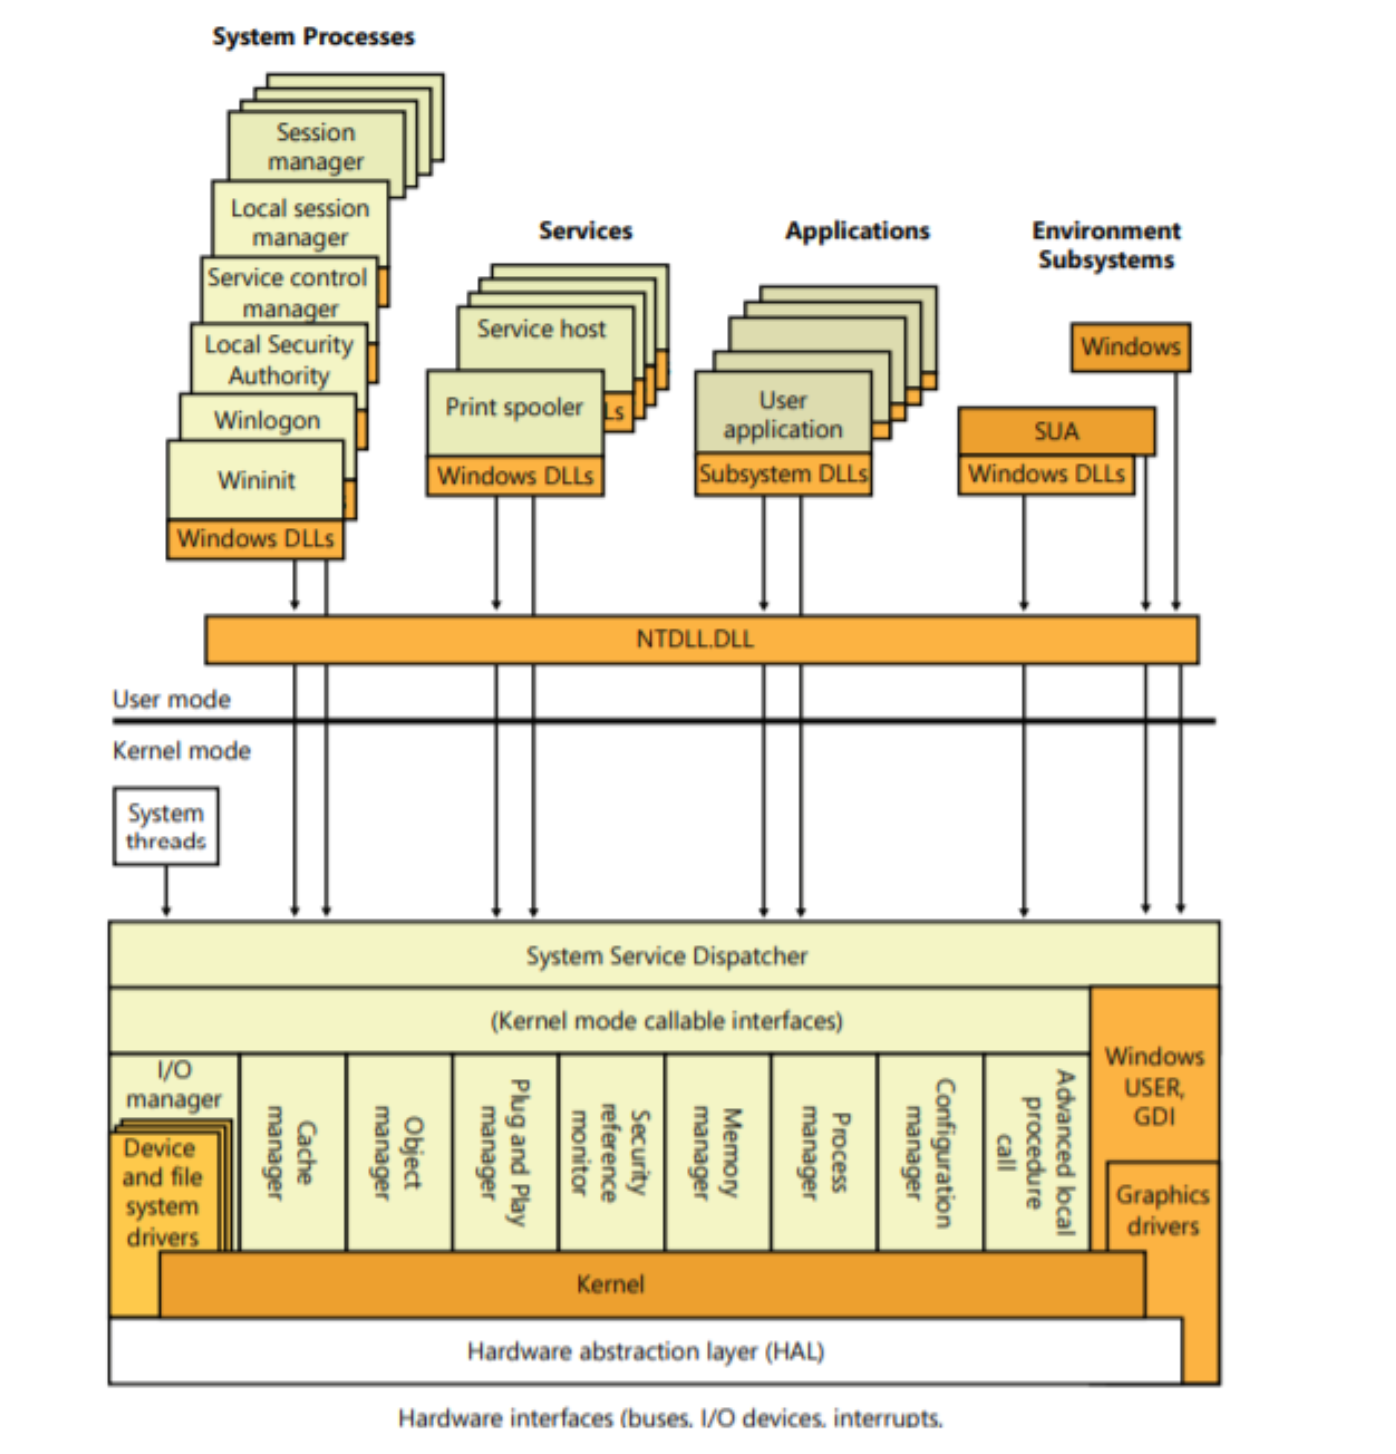
\includegraphics[width=12cm]{img/01_windows_schichten.png}
\end{center}


\paragraph{Client-Server-Modell}
\begin{itemize}
\item Diensterbringung durch eine zentrale Instanz
\item Client wendet sich mit Dienst-Wunsch an Server
\item Server erbringt gewünschten Dienst, wenn möglich
\item Mirkokern-Architekturen verwenden das Prinzip konsequent auf BS-Komponenten an
\item Beispiele: Speicherverwaltung im BS, NTP-Server, Drucker-Server
\end{itemize}

\end{document}










































